\documentclass[../report.tex]{subfiles}
\graphicspath{{\subfix{../image/}}}

\begin{document}

\subsection{Risk Assessment}
Engineers have the important responsibility to make sure that the products
they develop are safe and live up to the project goals. Therefore, a
risk assessment is an important part in each project. As this is a student/learning
project it makes sense to do two risk assessments. One for the project itself as a project (teamwork, workflow etc.) and one for the product (potential risks to 
operation and customer). The probabilities here were estimated as it is not in the scope of 
this project to make tests on multiple instances of the project/final product. Hence, the risk probabilities were estimated 
based on difficulties encountered during the development of the forklift and experiences
from previous semester projects.

The risk assessment for the group work will be shown now, as the countermeasures will essentially be 
explained on in the following paragraphs (Time management, Task management etc.).

So in this section the risk assessment for the team work will be discussed. The goal in the 
teamwork is to achieve a good learning outcome for all and to develop a satisfying workflow.
Important is also the adherence to the engineering method. Additionally, meeting deadlines is also
an important part, but this goes without saying.

\begin{figure}[h!]
    \centering
    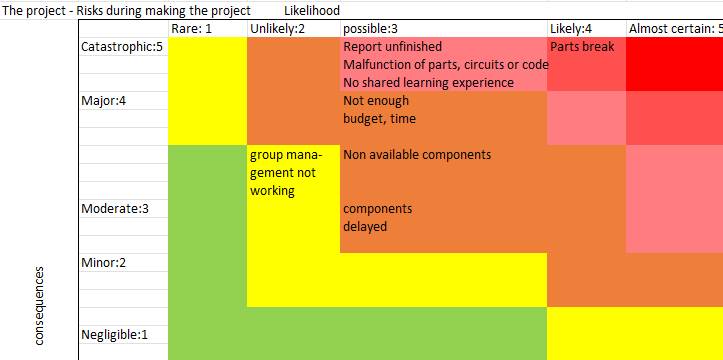
\includegraphics[width=1\textwidth]{risk_as_pro_ver1.png}
    \caption{Project risk assessment}
 \end{figure}

As can be seen - most of the risks come from bad team management and failed communication. For this reason, 
the following sections will elaborate on the team management and organization which have been 
worked out based on previous experiences.

\end{document}
